En este capítulo, se describe el \ref{pipeline} que sintetiza la metodología 
planificada para emplearse en las experimentaciones detalladas en capítulos 
subsiguientes. La Figura \ref{pipeline} muestra el pipeline propuesto 
para la ejecución de los experimentos.  \\\\

\begin{figure}[h!]
\includegraphics[width=0.85\textwidth]{images/Metodología.png}
\centering
\caption{Pipeline propuesto.  }
\label{pipeline}
\end{figure}

\section{\textit{Dataset}}

Para cada tipo de aplicación de ML, se tienen diferentes conjuntos de datos 
disponibles. Sin embargo, entre ellos es importante destacar que existen 
distintos tipos y se puede observar que algunos son más o menos 
complejos para ciertas tareas dependiendo del tamaño, número y la 
calidad de los datos.
\\\\
En el caso de la tarea de detección y clasificación de imágenes, 
se considera un \textit{dataset} de baja complejidad como aquel 
que contiene imágenes con objetos centrados, alineados en una sola 
dirección, con una resolución óptima y enfocados en el centro. Se ha 
demostrado en el marco teórico y en la revisión del estado del arte que 
este tipo de conjuntos de datos son fáciles de clasificar, 
especialmente para modelos como los mencionados en la sección \ref{arquitecturas}.
\\\\

En contraste, un conjunto de datos complejo difiere considerablemente de 
esta descripción. Las imágenes pueden contener varios objetos que no son 
los que se deben clasificar, presentando desalineación, baja resolución 
o falta de enfoque. Estas características dificultan que las redes 
neuronales convolucionales (CNN) logren una alta precisión, ya que no 
pueden aprender todos los patrones y realizar predicciones precisas para 
cada objeto. La Figura \ref{fig:combined} ilustra claramente la marcada 
diferencia entre estos dos tipos de conjuntos de datos.
\\\\
\begin{figure}
    \centering
    \subfloat[\centering Imagen de un \textit{dataset} ``poco complejo'' obtenido de \href{https://www.kaggle.com/datasets/giannisgeorgiou/fish-species}{\textit{Fish Species}}]{{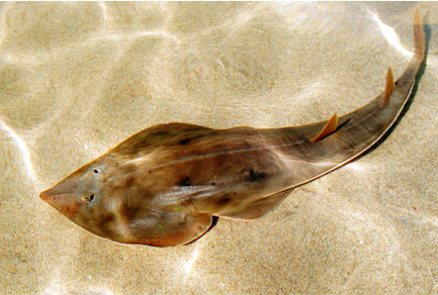
\includegraphics[width=4cm]{images/pezGuitarra.png} }}%
    \qquad
    \subfloat[\centering Imagen de un \textit{dataset} ``complejo'' obtenido de \href{https://www.kaggle.com/c/the-nature-conservancy-fisheries-monitoring}{\textit{The Nature Conservancy}}]{{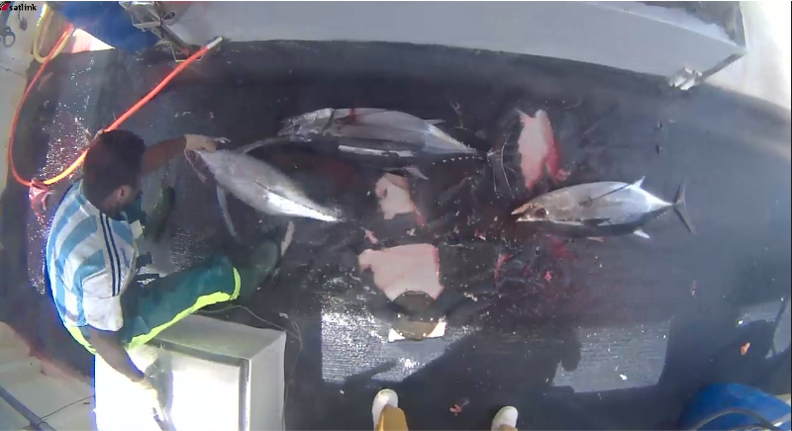
\includegraphics[width=5cm]{images/Bet.png} }}%
    \caption{Comparación de imágenes dentro de datasets diferentes}%
    \label{fig:combined}
\end{figure}
Además, los \textit{datasets} según su función de distribución de imágenes y 
el objetivo específico recaen en dos categorías. En la primera categoría, 
encontramos conjuntos de datos homogéneos y heterogéneos. Los \textit{datasets} 
homogéneos se caracterizan por 
tener la misma cantidad (o un número similar) de muestras por clase, lo que 
permite que los modelos aprendan de manera equitativa de cada clase. Sin embargo, 
esto no siempre refleja la realidad, donde la probabilidad de que aparezca una 
clase de objeto determinada puede ser mayor o menor que otra.
\\\\

En ese sentido, los \textit{heterogéneos} son aquellos que no tienen un 
número igual de muestras para cada clase. Esto puede ser intencional, ya que el 
creador del conjunto de datos diseñó la distribución de muestras de esa manera, o 
puede ser resultado de la falta de muestras disponibles.
\\\\
Además, los \textit{datasets} suelen venir etiquetados en relación a su objetivo. 
En nuestro caso, para entrenar una CNN, se dispone de un repositorio de imágenes 
junto, cada una dentro de una carpeta con el nombre de su respectiva clase. En 
cambio, para entrenar una red como YOLO, se requieren los ``bounding boxes'' que 
delimitan la ubicación de los objetos.
\\\\
Dado que encontrar un \textit{dataset} de imágenes etiquetadas de peces resulta 
inviable para el caso peruano, se han utilizado dos tipos de conjuntos de datos 
encontrados en la plataforma Kaggle para esta investigación. Ambos conjuntos contienen 
imágenes y sus respectivas etiquetas, pero uno presenta peces centrados y sin ruido, 
mientras que el otro incluye fotografías tomadas en un entorno real donde se encuentran 
peces, personas e instrumentos de pesca, lo que lo convierte en un conjunto de datos 
heterogéneo. El primero se utilizará para realizar comparaciones entre los modelos, 
mientras que el segundo se empleará para el entrenamiento y prueba del pipeline final.
\\\\
Estas imágenes fueron re-dimensionadas dependiendo del tamaño de entrada que se espera 
para cada red, y luego fueron pasadas al clasificador.

\section{Detector}
Para la detección de cada imagen del \textit{dataset}, se utilizó un módulo de detección 
basado en YOLO v5, el cual ya ha sido preentrenado con el conjunto de datos ``Objects365'', 
brindando la capacidad de detectar la categoría de peces. Además, se entrenó un YOLO v5 con 
el \textit{dataset}, ignorando las clases detectadas. Por último, también utilizaremos un 
modelo llamado UniDet, el cual ha sido entrenado con los \textit{datasets} ``Objects365'', 
``OpenImages'' y ``COCO''.  Una vez que las imágenes sean procesadas por el detector, 
esperamos obtener \textit{los bounding boxes} donde se encuentren los peces individualmente. 
Se puede visualizar este proceso en la figura \ref{fig:detector_pez}.
\begin{figure}[h!]
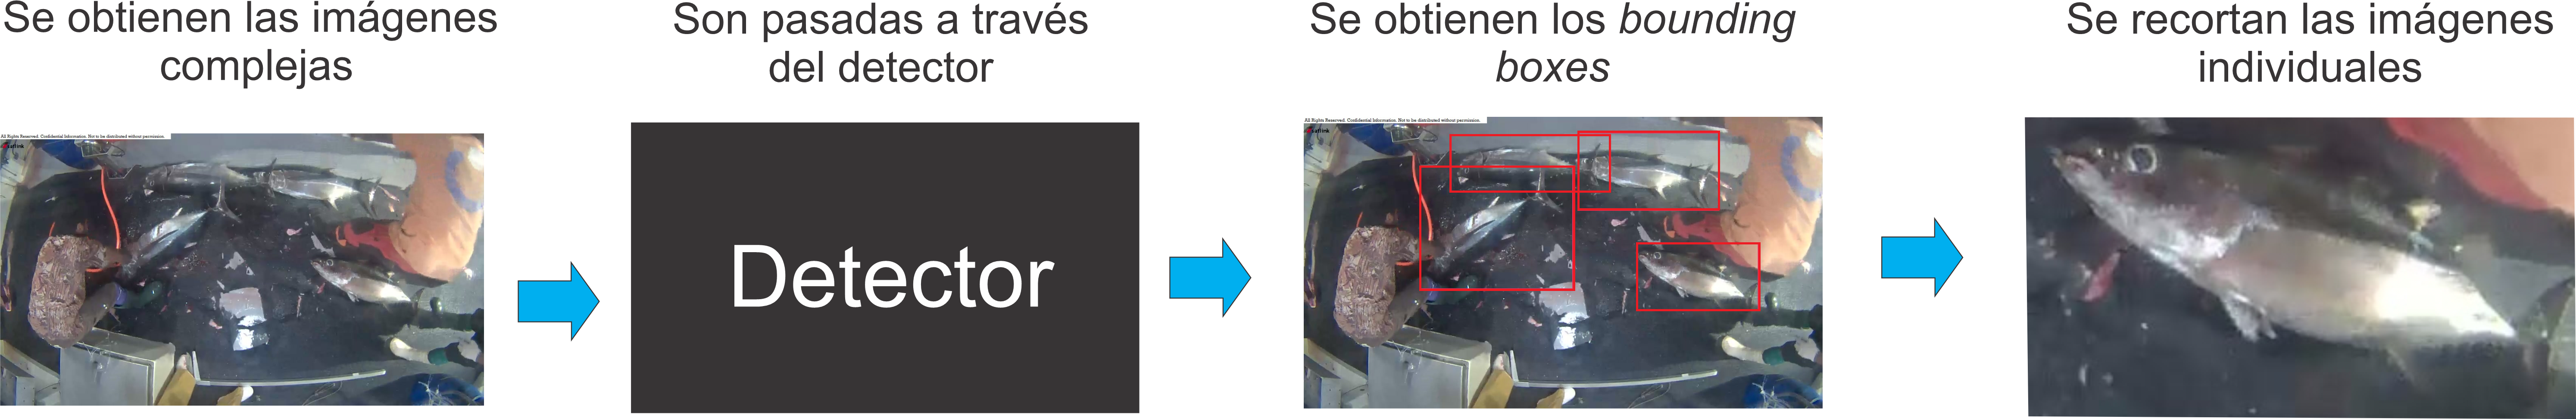
\includegraphics[width=1\textwidth]{images/detector_pez.png}
\caption{Flujo de entrada y salida del detector }
\label{fig:detector_pez}
\end{figure}



\section{Clasificador}
Una vez ubicados los peces, se recortó y redimensionó las imágenes 
para ocupar la entrada que espera el clasificador. Para los experimentos, se 
utilizó la resolución específica para cada una de las redes a probar. Estas 
redes también fueron obtenidas con sus pesos pre-entrenados con 
``Imagenet". Se les aplicó TL, congelando todas las capas convolucionales. Por 
último, a cada uno de estos modelos se le añadió una capa llamada 
``\textit{GlobalAveragePooling}'' y unas nuevas capas clasificadoras. Esto tuvo 
la finalidad de disminuir el número de parámetros 
finales de la capa de clasificación, mejorar su precisión y reducir su tiempo 
de entrenamiento. El flujo se ve evidenciado en la imagen \ref{fig:clasificador_pez}.

\begin{figure}[h!]
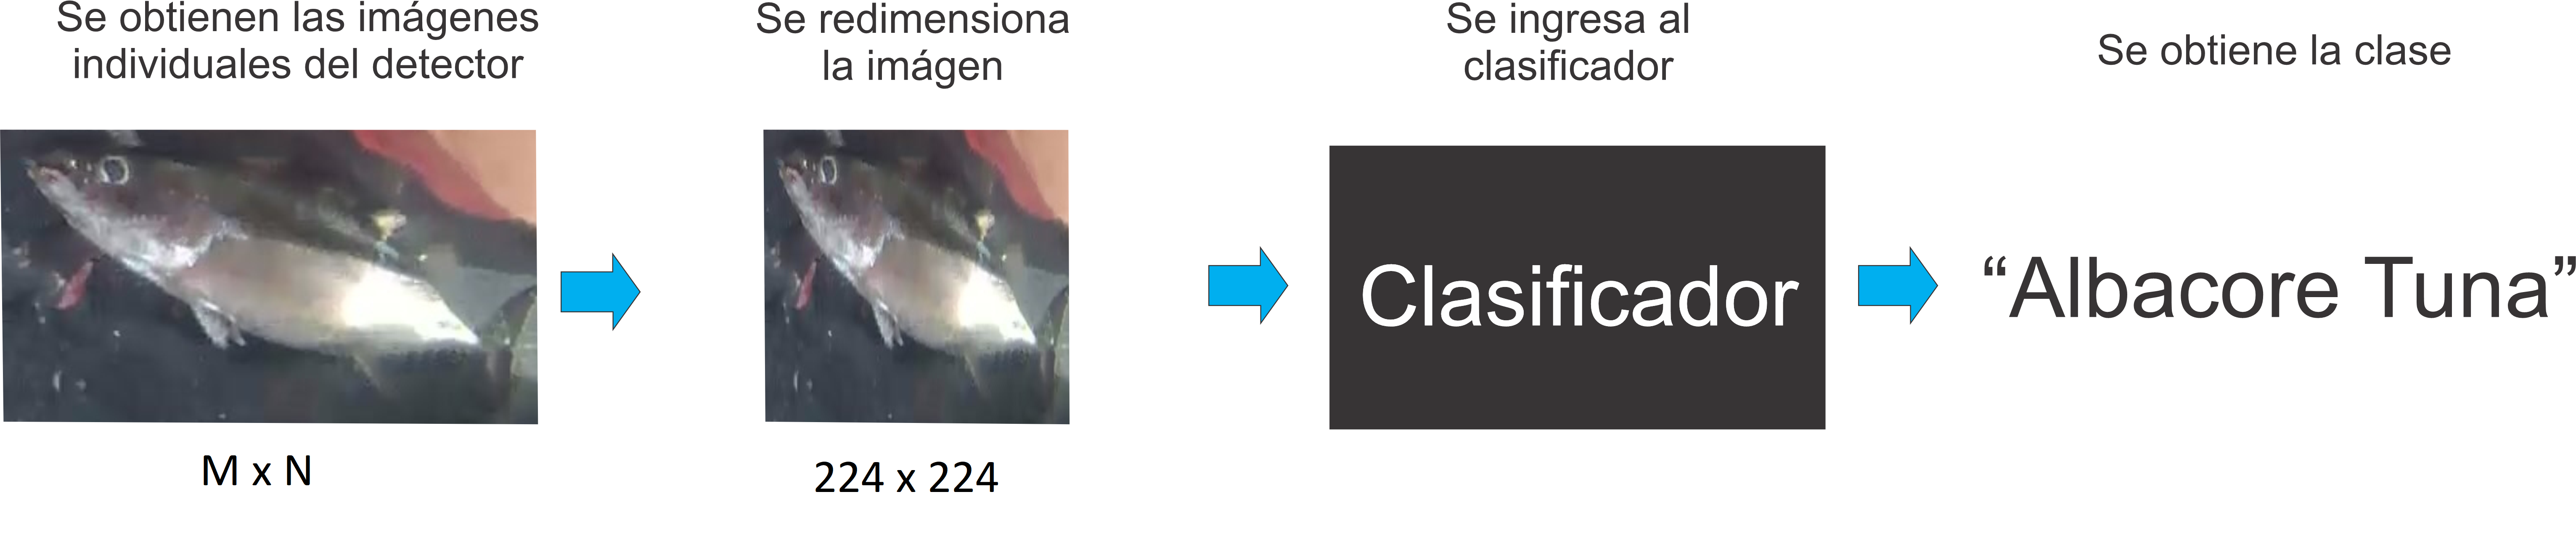
\includegraphics[width=1\textwidth]{images/clasificador_label.png}
\caption{Flujo de entrada y salida del clasificador }
\label{fig:clasificador_pez}
\end{figure}


\subsection{Evaluación de clasificadores para la experimentación}
En 2020, Orhan Yalsin \cite{DataModelos} realizó una resumen con algunas métricas para la 
evaluación de diferentes modelos de vanguardia, los cuales son mostrados 
en la tabla \ref{evaluación}. Nos basamos en sus resultados para seleccionar 
aquellos modelos que son mas eficientes tanto en tiempo, espacio y precisión.

\begin{table}[h!]
    \begin{tabular}{|l|r|r|r|r|r|}
    \hline
    \textbf{Model}                                               & \multicolumn{1}{l|}{\textbf{Size}} & \multicolumn{1}{l|}{\textbf{\begin{tabular}[c]{@{}l@{}}Top-1 \\ Accuracy\end{tabular}}} & \multicolumn{1}{l|}{\textbf{\begin{tabular}[c]{@{}l@{}}Top-5 \\ Accuracy\end{tabular}}} & \multicolumn{1}{l|}{\textbf{Parameters}} & \multicolumn{1}{l|}{\textbf{Depth}} \\ \hline
    Xception                                                     & 88 MB                              & 0.790                                                                                   & 0.945                                                                                   & 22,910,480                               & 126                                 \\ \hline
    VGG16                                                        & 528 MB                             & 0.713                                                                                   & 0.901                                                                                   & 138,357,544                              & 23                                  \\ \hline
    VGG19                                                        & 549 MB                             & 0.713                                                                                   & 0.900                                                                                   & 143,667,240                              & 26                                  \\ \hline
    ResNet50                                                     & 98 MB                              & 0.749                                                                                   & 0.921                                                                                   & 25,636,712                               & -                                   \\ \hline
    ResNet101                                                    & 171 MB                             & 0.764                                                                                   & 0.928                                                                                   & 44,707,176                               & -                                   \\ \hline
    ResNet152                                                    & 232 MB                             & 0.766                                                                                   & 0.931                                                                                   & 60,419,944                               & -                                   \\ \hline
    ResNet50V2                                                   & 98 MB                              & 0.760                                                                                   & 0.930                                                                                   & 25,613,800                               & -                                   \\ \hline
    ResNet101V2                                                  & 171 MB                             & 0.772                                                                                   & 0.938                                                                                   & 44,675,560                               & -                                   \\ \hline
    ResNet152V2                                                  & 232 MB                             & 0.780                                                                                   & 0.942                                                                                   & 60,380,648                               & -                                   \\ \hline
    InceptionV3                                                  & 92 MB                              & 0.779                                                                                   & 0.937                                                                                   & 23,851,784                               & 159                                 \\ \hline
    \begin{tabular}[c]{@{}l@{}}Inception\\ ResNetV2\end{tabular} & 215 MB                             & 0.803                                                                                   & 0.953                                                                                   & 55,873,736                               & 572                                 \\ \hline
    MobileNet                                                    & 16 MB                              & 0.704                                                                                   & 0.895                                                                                   & 4,253,864                                & 88                                  \\ \hline
    MobileNetV2                                                  & 14 MB                              & 0.713                                                                                   & 0.901                                                                                   & 3,538,984                                & 88                                  \\ \hline
    DenseNet121                                                  & 33 MB                              & 0.750                                                                                   & 0.923                                                                                   & 8,062,504                                & 121                                 \\ \hline
    DenseNet169                                                  & 57 MB                              & 0.762                                                                                   & 0.932                                                                                   & 14,307,880                               & 169                                 \\ \hline
    DenseNet201                                                  & 80 MB                              & 0.773                                                                                   & 0.936                                                                                   & 20,242,984                               & 201                                 \\ \hline
    NASNetMobile                                                 & 23 MB                              & 0.744                                                                                   & 0.919                                                                                   & 5,326,716                                & -                                   \\ \hline
    NASNetLarge                                                  & 343 MB                             & 0.825                                                                                   & 0.960                                                                                   & 88,949,818                               & -                                   \\ \hline
    EfficientNetB0                                               & 29 MB                              & 0.771                                                                                   & 0.933                                                                                   & 5,330,571                                & -                                   \\ \hline
    EfficientNetB1                                               & 31 MB                              & 0.791                                                                                   & 0.944                                                                                   & 7,856,239                                & -                                   \\ \hline
    EfficientNetB2                                               & 36 MB                              & 0.801                                                                                   & 0.949                                                                                   & 9,177,569                                & -                                   \\ \hline
    EfficientNetB3                                               & 48 MB                              & 0.816                                                                                   & 0.957                                                                                   & 12,320,535                               & -                                   \\ \hline
    EfficientNetB4                                               & 75 MB                              & 0.829                                                                                   & 0.964                                                                                   & 19,466,823                               & -                                   \\ \hline
    EfficientNetB5                                               & 118 MB                             & 0.836                                                                                   & 0.967                                                                                   & 30,562,527                               & -                                   \\ \hline
    EfficientNetB6                                               & 166 MB                             & 0.840                                                                                   & 0.968                                                                                   & 43,265,143                               & -                                   \\ \hline
    EfficientNetB7                                               & 256 MB                             & 0.843                                                                                   & 0.970                                                                                   & 66,658,687                               & -                                   \\ \hline
    \end{tabular}
    \caption{Evaluación de diferentes modelos. Tabla brindada por Orhan Yalcin \protect\cite{DataModelos}. }
    \label{evaluación}
\end{table}

\\\\
Esta tabla destaca varios modelos notables por su equilibrio entre 
tamaño, cantidad de parámetros y precisión. Entre ellos VGG19 
(si consideramos solo las capas convolucionales), ResNet50, InceptionV3, 
y los EfficientNetBX resultan tener una buena relación entre el peso, el 
número de parámetros y la precisión que estas obtienen, esta última 
siendo de las más altas dentro de todos estos modelos. Se tuvo en 
consideración la ejecución en videos en tiempo real y por ello se necesitó 
que el modelo sea el más pequeño posible evitando perder la precisión. Por 
otra parte, están las MobileNet, las cuales ya han sido utilizadas para el 
procesamiento de imágenes en tiempo real por ser más ligeras, enfocadas a 
ser utilizadas en celulares. Creemos que todas estas redes eran aptas para 
este problema y pasarán a ser evaluadas en el siguiente capítulo, en base 
al primer \textit{dataset} mencionado anteriormente. \\\\
Una vez analizado esas redes en base al \textit{dataset}, se compararon 
la precisión y costo entre ellas y se obtuvo la que finalmente pasará a 
formar parte del \textit{pipeline} final, en donde fue encargada de 
clasificar cada imagen obtenida por la red Yolo.\\\\
En el siguiente capítulo finalmente se verá la experimentación realizada con todos 
los modelos anteriormente señalados, tanto como la especificación de las 
imágenes y la experimentación del \textit{pipeline} final.

\section{\textit{Labeled Boxes}}
Una vez generadas las etiquetas del clasificador para cada una de las 
imágenes obtenidas por el detector, se procedió a asignar cada 
\textit{bounding box} con su etiqueta correspondiente. Terminado este 
trabajo, se obtuvo como salida la imagen con los \textit{labeled boxes} 
para cada instancia de pez que se encuentre. 

\begin{figure}[h!]
    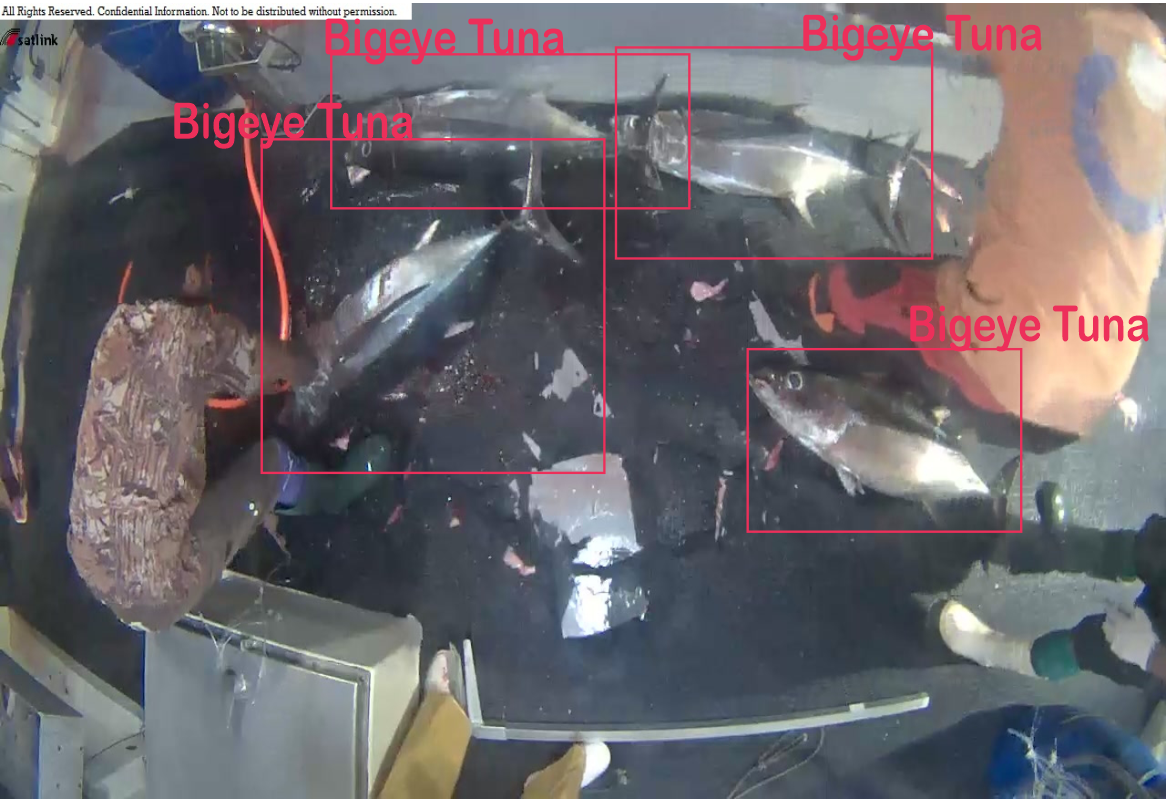
\includegraphics[width=1\textwidth]{images/BoundingBox.png}
    \caption{\textit{Labeled Boxes} dentro de la imagen ya procesada. }
    \label{fig:LabelBoxes}
\end{figure}
